\documentclass[11pt]{article}

%------------------------------------------------------------------------
\usepackage{geometry}
\usepackage{latexsym}
\usepackage[empty]{fullpage}
\usepackage{titlesec}
\usepackage[parfill]{parskip}
\usepackage{marvosym}
\usepackage[usenames,dvipsnames]{color}
\usepackage{verbatim}
\usepackage{enumitem}
\usepackage[hidelinks]{hyperref}
\usepackage{fancyhdr}
\usepackage{lineno}
\usepackage{lastpage}
\usepackage{lipsum}
\usepackage{graphicx}
\usepackage{color}
\usepackage{setspace}
\usepackage{ragged2e}
\usepackage{tikz}
\usepackage{hyperref}
\usepackage[capitalise]{cleveref}
%\usepackage[bitstream-charter]{mathdesign} % for journal-like fonts
\usepackage{url}
\hypersetup{colorlinks,linkcolor=blue,urlcolor=blue}
\urlstyle{ttfamily}
\usepackage[superscript]{cite}
\usepackage{microtype}
\renewcommand\citeform[1]{[#1]}

\graphicspath{{./figures/}}
%------------------------------------------------------------------------
% Paper margin setup
 \geometry{
 letterpaper,
 total={216mm,280mm},
 left=24mm,
 right=24mm,
 top=20mm,
 bottom=20mm
 }
 
\definecolor{idl}{RGB}{0,255,0}
\definecolor{skp}{RGB}{255,200,0}
\definecolor{mlt}{RGB}{255,0,0}
 
\newcommand\hflink[1]{\hyperref[#1]{Fig.~\!\ref*{#1}}} 

\setlength{\abovecaptionskip}{0pt} 
\setlength{\belowcaptionskip}{0pt} 

%-----------------------------------------------------------------------
\pagestyle{fancy}
\fancyhf{} 

\lfoot[<even output>]{\color{Gray} Research interests}
\cfoot[<even output>]{\color{Gray}Page \thepage\ of \pageref{LastPage}}
\rfoot[<even output>]{\color{Gray}S. Sunoj}

\renewcommand{\headrulewidth}{0pt}
\renewcommand{\footrulewidth}{0pt}

\urlstyle{same}

\raggedbottom
\raggedright
\setlength{\tabcolsep}{0in}
%------------------------------------------------------------------------
\newcommand\idea[1]{{\bfseries #1}\\}

\titleformat{\section}
  {\large\bfseries}{\thesection.}{0.7em}{\vspace{-0.5em}} 

\titleformat{\subsection}
  {\normalfont\bfseries}{\thesubsection. }{0.2em}{\vspace{-0.7em}}

\titleformat{\subsubsection}
  {\normalfont}{\thesubsubsection.}{0em}{\vspace{-1.2em}} 


\begin{document}
\begin{center}
\hrule
%\vspace{0.5em}
{\Large\textbf{Statement of research interest and vision}}\\
\vspace{0.5em}
\normalsize{Sunoj Shajahan\\
Postdoctoral Associate, Nutrient Management Spear Program,\\
Cornell University, Ithaca, NY.}
\vspace{0.5em}
\hrule
\end{center}
\vspace{0.5em}
\justify
\setstretch{1.15}
\hspace{1.5em} My research interest aligns with \textbf{one of the four foundational focus areas, Digital Agriculture and Advanced Analytics in K-State's plan for economic prosperity}. Over the past 6 years, I have been using advanced data analytics on multi-source geospatial data and developing data-driven decision support tools for agriculture in near real-time. I have been \textbf{fascinated and involved in using free and open-source software (FOSS)} platforms and developing automated workflows and tools.~Among the several technologies in agriculture, the \textbf{slower adoption of information-intensive technologies}, such as yield monitors, variable rate technologies, remotely sensed imagery or general imagery is reported to be most likely due to the complexity involved in transforming data into valuable information (\href{https://agecon.unl.edu/cornhusker-economics/2017/precision-agriculture-adoption-profitability}{Study1}, \href{https://www.emerald.com/insight/content/doi/10.1108/AFR-11-2019-0121/full/html}{Study2}).~Even though many commercial software applications are available, not all farmers benefit from it, because they are either complicated to use, expensive, and would require additional skills or training to get value from the data. In such scenarios, \textbf{user-friendly tools developed from FOSS platforms will most likely improve the adoption of technologies}. 

%My research interest is on using advanced data analytics on multi-source geospatial data and developing data-driven decision support tools for agriculture in near real-time, which aligns with \textbf{one of the four foundational focus areas in K-State's plan for economic prosperity}. 


%My research interest is on developing digital image processing tools and data-driven decision support tools for precision agriculture applications. Among the several technologies in precision agriculture, the adoption of digital imagery ranks low, because of the complexity involved in interpreting useful information from the images  \href{https://agecon.unl.edu/cornhusker-economics/2017/precision-agriculture-adoption-profitability}{(Link)}.  Even though many commercial image processing applications are available, not all farmers benefit from it, because they are either  sophisticated to use or expensive. In such scenarios, user-friendly tools developed from ``open source platforms'' will invite more farmers to adopt technology and allow researchers to share findings with farmers. 

%\vspace{-0.5em}\hspace{1.5em} My research philosophy is to use free and open source software (FOSS) platforms (e.g., ImageJ, R, Python, OpenCV, QGIS) for research and tool development, so that my contributions will be accessible to the farmers and reproducible across researchers around the world. Two other reasons to use open source platforms include: (1) It increases adoption of precision agriculture technology among farmers, as the algorithms I develop can be freely used by the farmer, unlike the commercial software that comes with expensive license and renewal; and (2) It ensures ``data security'', as the software tool and the data will remain in the farmer's system, unlike the commercial software where the farmer may have to upload the data to cloud-based platforms. 

%\hspace{1.5em} In precision agriculture, the adoption rate of imagery ranked 8 out of 10 technologies, because the farmers lack the knowledge to work on images and interpret useful information \href{https://agecon.unl.edu/cornhusker-economics/2017/precision-agriculture-adoption-profitability}{(Link)}. Even though many commercial image processing applications are available, but does not benefit all farmers because they are either  sophisticated to use or expensive. In such a scenario, algorithms from open source platforms will welcome more farmers to adopt the  technology and researchers can immediately share the findings to farmers. 

\vspace{-0.5em}\hspace{1.5em} In my current position at Cornell, I have been involved in direct discussions with farmers and farm consultants, and the same question being asked ``\textbf{how can we use your findings?}'' For example, in one of my recent publications \href{https://link.springer.com/article/10.1007/s11119-021-09793-z}{(Link)}, we tested various spatial estimation methods in R software and determined that the `Matern kriging' approach produces the lowest error in generating a smooth raster map from the yield monitor data. This raster data layer serves as an input to develop their yield stability zones (from multi-year yield data). However, this approach/workflow is currently available only on the R platform, and not in any other geographic information system software. Therefore, I worked on packaging the code into a tool and implementing it as a QGIS\footnote{Free and open-source geographic information system} plugin. This enables farmers to use the tool with `click \& run' features with their own farm data. 

\vspace{-1em}
\section{Current research works:}\vspace{-0.3em}
%My doctoral and postdoctoral research projects and accomplishments are as follows: \vspace{-0.5em}
\begin{itemize}[leftmargin=0.4cm, itemsep = -0.7em]
\item Developing recurrent neural network framework with a time series UAS\footnote{Unmanned aerial systems} imagery to predict corn grain and silage yield across many fields in New York. \href{https://www.esf.edu/stratus/stratus-2022-5-23.pdf}{(Page 35; Link)}
\item Using satellite imageries of corn grain and silage fields and trained random forest models to identify low and high yielding areas in field and compared with the yield monitor data \href{https://nnyagdev.org/wp-content/uploads/2021/02/NNYADPSatelliteDroneReportFINAL.pdf}{(Link)}.
\item Using multispectral UAS imagery to estimate the actual yield (in bu/ac or Mg/ha) to use it as a proxy to the yield monitor data \href{https://www.mdpi.com/2072-4292/13/19/3948}{(Link)}.
%\item Extensive data munging and processing for predictive model development, automated analysis pipeline development, and visualization
%\item Developed a standalone plugin for ImageJ (FOSS) to identify plant rows, count plant stands, and evaluate plant spatial distribution from high-resolution UAS imagery (manuscript submitted)
%\item Quantifying the plant spatial distribution from UAS imagery to evaluate the spacing uniformity and developed a unique index to measure spacing uniformity
%\item Developed digital image analysis algorithm based on shape features to count soybean aphids, exoskeletons, and leafspots in soybean trifoliate (Received 3 research awards; \href{https://elibrary.asabe.org/abstract.asp?aid=48461}{Link}) 
%\item Using shape features to identify and classify weed species from weed mixtures 
%\item Developing simple 3D reconstruction algorithm based on engineering drawing principles for lab-based plant phenotyping  
%\item As listed in my CV, I have 18 peer-reviewed publications (to date), 14 proceedings/extension articles, 45 conference presentations, 5 extension presentations, and 4 research paper awards that attest to the quality of my research activities and accomplishments.
\end{itemize}


\vspace{-1em}
\section{Research vision:}\vspace{-0.5em}
\textls[-10]{Aligning my expertise on using geospatial data layers and \textbf{K-State's focus on Digital Agriculture and Advanced Analytics}, my vision is to explore:}

\vspace{-0.5em}
\begin{itemize}[leftmargin=0.4cm, itemsep = -0.7em]
\item \textbf{Digital twin in agriculture} -- \textls[-10]{The concept of a digital twin has been infiltrating agriculture at a slow pace, but not much has been accomplished. Agriculture has emerged to be one of the platforms where a huge amount of data are being collected on a daily basis through satellites, farm equipment, weather networks, soil scanning sensors, and weekly UAS flights (\cref{fig1}). These geospatial data layers could be fused to obtain a big dataset (combined over multiple years and farms). This dataset can be used to develop artificial intelligence models and build a ``digital twin'' model for predictive and prescriptive analytics. The Kansas state is known for its \textbf{variability in climatic and production conditions}, where a framework developed could be scaled and translated across the nation.} 

\vspace{-0.6em}
\begin{figure}[h]
\centering 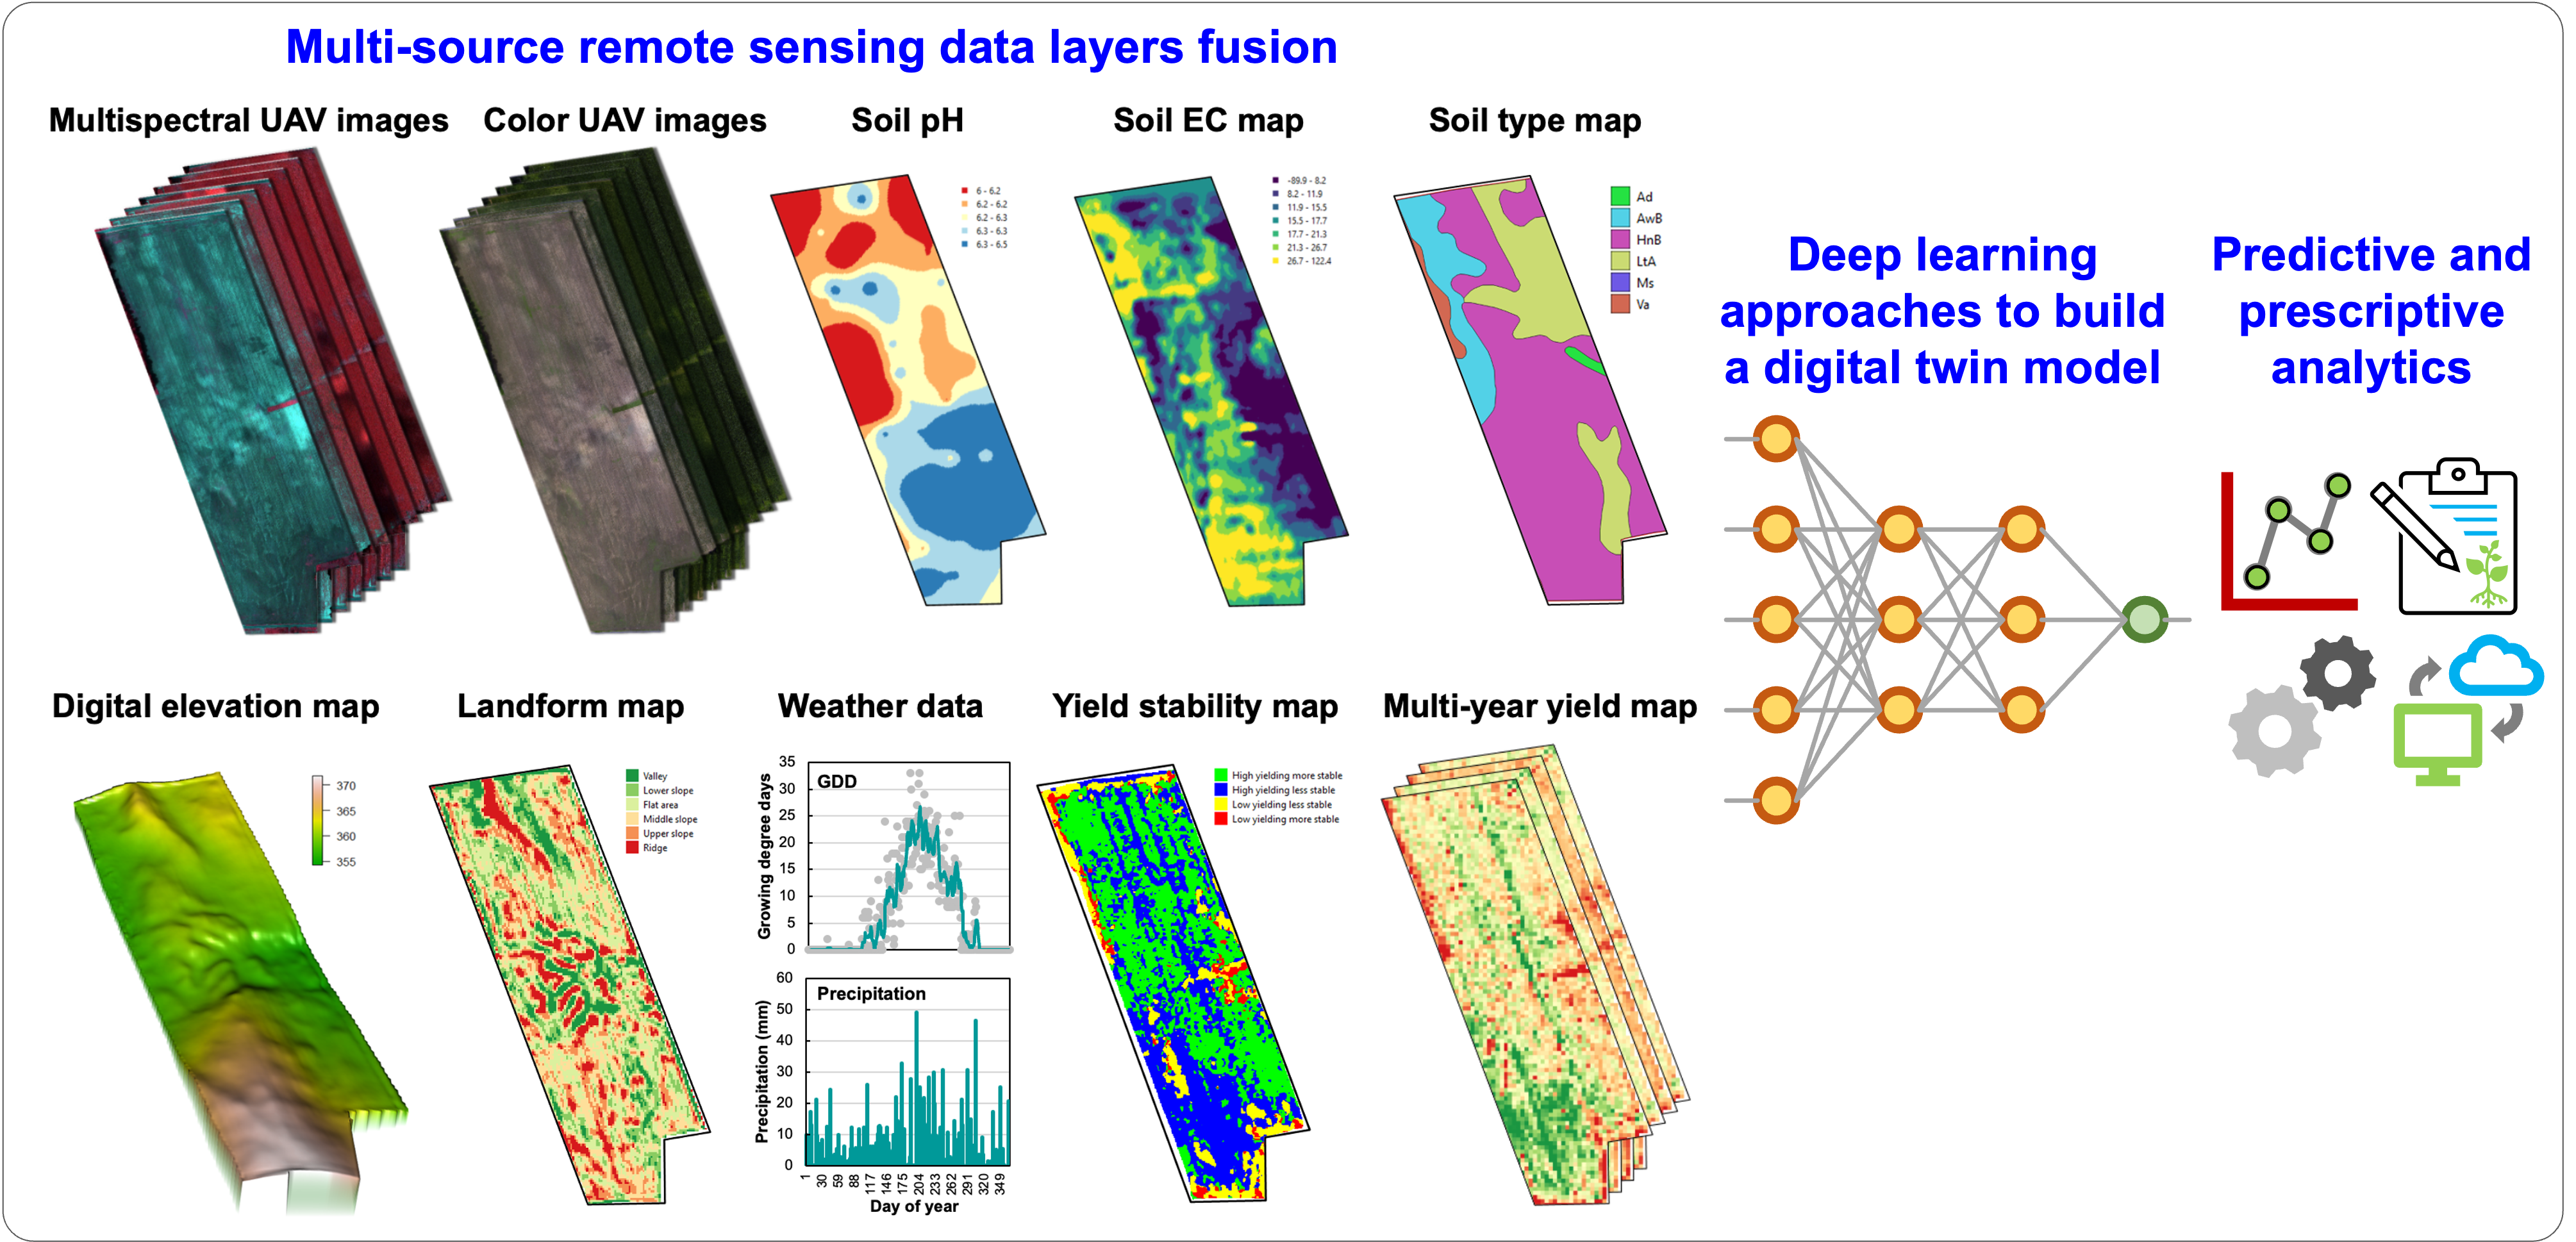
\includegraphics[width=0.97\textwidth]{PlanFig2.png} \\
\caption{Illustration of using multi-source geospatial data and developing a digital twin model for predictive and prescriptive analytics.}
\label{fig1}
\end{figure}

\item \textbf{Yield stability zone development:} \textls[-10]{Within field yield stability zones ,developed from multi-year yield data, let the farmer understand high and low yielding areas within the field; therefore, it is one of the important layers that would \textbf{help in implementing site-specific management}. Currently, yield monitor data is being used to create stability zones, but I would like to explore if remotely sensed images could be used for delineating these zones, which could be expanded to a larger scale.}

\item \textbf{Tools for on-farm research:} \textls[-10]{Precision agriculture technologies help in conducting on-farm research experiments capturing the variability in the field; however, analyzing the data and transforming the data into valuable information is not straightforward. I am interested in working with farmers and farm consultants in developing tools that would help in conducting on-farm research.}
\end{itemize}

%--------------------------------------------------------------------
\vspace{-1em}
\section{Collaboration}\vspace{-0.5em}
\hspace{1.5em} \textls[0]{I believe collaboration is an effective way to solve agricultural problems and provide adequate solutions. In my current position at Cornell, I have collaborated with faculties from other departments and universities and been exposed to writing collaborative grants. I aim to continue conducting interdisciplinary research with scientists in agronomy, agricultural economics, and biological and agricultural engineering, as well as researchers from other universities in the state.} 

%--------------------------------------------------------------------
\vspace{-1em}
\section{Funding}\vspace{-0.5em}
\hspace{1.5em} I have gained experience in writing small ($\approx$\,\$34\,000) to medium ($\approx$\,\$1.2 million) scale research proposals in the area of precision agriculture for funding programs such as NESARE, USDA-NIFA, NSF, and local funding programs. Some of these were successful grants and the others gave me a good experience. I will seek funding opportunities from the state and federal funding agencies. Also, I will seek collaborations and funding support from industries and agricultural stakeholders.

%--------------------------------------------------------------------
%\newpage
%\bibliographystyle{unsrt}
%\bibliography{mypublications}

\end{document}